% !TEX TS-program = pdflatex
% !TEX encoding = UTF-8 Unicode

% This is a simple template for a LaTeX document using the "article" class.
% See "book", "report", "letter" for other types of document.

\documentclass[11pt]{article} % use larger type; default would be 10pt

\usepackage[utf8]{inputenc} % set input encoding (not needed with XeLaTeX)

%%% Examples of Article customizations
% These packages are optional, depending whether you want the features they provide.
% See the LaTeX Companion or other references for full information.

%%% PAGE DIMENSIONS
\usepackage{geometry} % to change the page dimensions
\geometry{letterpaper} % or letterpaper (US) or a5paper or....
% \geometry{margins=2in} % for example, change the margins to 2 inches all round
% \geometry{landscape} % set up the page for landscape
%   read geometry.pdf for detailed page layout information

\usepackage{graphicx} % support the \includegraphics command and options

% \usepackage[parfill]{parskip} % Activate to begin paragraphs with an empty line rather than an indent

%%% PACKAGES
\usepackage{booktabs} % for much better looking tables
\usepackage{array} % for better arrays (eg matrices) in maths
\usepackage{paralist} % very flexible & customisable lists (eg. enumerate/itemize, etc.)
\usepackage{verbatim} % adds environment for commenting out blocks of text & for better verbatim
\usepackage{subfig} % make it possible to include more than one captioned figure/table in a single float
\usepackage{hyperref}
% These packages are all incorporated in the memoir class to one degree or another...

%%% HEADERS & FOOTERS
\usepackage{fancyhdr} % This should be set AFTER setting up the page geometry
\pagestyle{fancy} % options: empty , plain , fancy
\renewcommand{\headrulewidth}{0pt} % customise the layout...
\lhead{}\chead{}\rhead{}
\lfoot{}\cfoot{\thepage}\rfoot{}

%%% SECTION TITLE APPEARANCE
\usepackage{sectsty}
\allsectionsfont{\sffamily\mdseries\upshape} % (See the fntguide.pdf for font help)
% (This matches ConTeXt defaults)

%%% ToC (table of contents) APPEARANCE
\usepackage[]{tocbibind} % Put the bibliography in the ToC
\usepackage[titles,subfigure]{tocloft} % Alter the style of the Table of Contents
\renewcommand{\cftsecfont}{\rmfamily\mdseries\upshape}
\renewcommand{\cftsecpagefont}{\rmfamily\mdseries\upshape} % No bold!

%%% Setup hyperlinks %%%
\hypersetup{
  colorlinks = true,
  linkcolor = blue
}

%%% END Article customizations

%%% The "real" document content comes below...

\title{VEGAS \\ \Large HPC Software Developer Documentation}
\author{Simon Scott, UC Berkeley\\Jayanth Chennamangalam, WVU}
%\date{} % Activate to display a given date or no date (if empty),
         % otherwise the current date is printed 

\begin{document}
\maketitle
\parskip 7.2pt

\tableofcontents
\clearpage

%%%%%%%%%%%%%%%%%%%%%%%%%%%%%%%%%%%%%%%%%%%%%
% CHAPTER: OVERVIEW
%%%%%%%%%%%%%%%%%%%%%%%%%%%%%%%%%%%%%%%%%%%%%
\section{VEGAS Overview: ROACHs and HPCs}

\subsection{Introduction}

This section provides an overview of the operation of the ROACHs and HPCs. Since the operation of the ROACH boards is beyond the scope of this document, only those details necessary to understand how the ROACH boards interface with the HPC will be provided.

The ROACH boards can operate in 17 different observing modes. These modes can be divided into two categories: high bandwidth ($\ge$ 250 MHz) and low bandwidth ($<$ 250MHz). In high-bandwidth modes, the ROACH FPGA board acts as a spectrometer, calculating the Fourier Transform of the sampled IF waveform, integrating, and sending the integrated spectrum to the HPC (CPU and GPU) for post-processing and storage. In low-bandwidth modes, the FPGA board simply downconverts and packetizes the IF waveform, before sending it to the HPC. The HPC cluster computes the Fourier Transform on GPUs, before writing to disk.

\subsection{Control and Timing Inputs to the ROACH}

Each ROACH has four control inputs:
\begin{itemize}
\item 1 calibration switching signal
\item 2 position/frequency switching signals
\item 1 blanking signal
\end{itemize}
And two timing inputs:
\begin{itemize}
\item 1 PPS (1 pulse per second)
\item ARM (indicates when FPGA must start integrating spectra)
\end{itemize}

The calibration switching signal and the two position/frequency switching signals are collectively known as the ``switching signals''. These three signals allow the spectrometer to operate in eight different ``switching states''. Note that although the ARM signal is regarded as an electrical signal in this document, it is actually implemented as a register on each of the ROACH FPGAs. This register is set by sending an appropriate Ethernet packet to the ROACH.

\subsection {Operation of the ROACH}

\subsubsection {Operation in High-Bandwidth Modes}

The FPGA spectrometers are ``free running''; they are never started or stopped. The starting and stopping of the integrations is implemented by the HPC software. The FPGA performs an initial, fixed-period integration (on the order of 1ms), in order to reduce the datarate. The integrated spectrum is then sent to the CPU/GPU for longer integration.

The FPGA spectrometer integrates spectra and counts the number of spectrum in an integration. Each integration ends when a maximum number of spectra (called FPGA\_NMAX\_SPECTRA) is reached, or when one of the switching signals change. In either of these cases, the integration stops at the next spectral boundary, and the integrated spectrum is transmitted to the HPC over the 10Gbe link. The next integration begins immediately.

If the blanking signal goes active at any point, the current spectrum (as outputted from the PFB) will be included in the integration performed on the FPGA, but all subsequent spectra will not be added to the vector accumulators (i.e. will not be integrated) until the blanking signal is cleared. This means that the blanking signal is re-registered to the next spectral boundary on the FPGA.

In summary, while the blanking signal is high, no spectra are added to the vector accumulators on the FPGA, and the counter that counts the number of spectra in the current integration is not incremented.

FPGA\_NMAX\_SPECTRA will typically be set so that the FPGA integrates 1 millisecond worth of spectra before sending the spectra to the CPU/GPU for further integration.

\subsubsection {Operation in Low-Bandwidth Modes}

The FPGA is again ``free-running''. The starting and stopping of the integrations is implemented by the HPC. The FPGA simply performs the necessary digital-downconversion and filtering on the sampled waveform before packetising the data and sending it to the HPC. No spectroscopy is performed in these modes.

Unlike the high-bandwidth mode, the FPGA still sends samples to the HPC when the blanking signal is active. However, when the blanking signal is active, the FPGA sets the blanking bit in the header of the packets sent to the HPC. This informs the HPC that the blanking signal is active and that the spectrum that is currently being computed on the HPC must not be added to the vector accumulators (in the HPC).

\subsubsection{Instructing the HPC to Start Integrating}

When the FPGA is powered up, the SPEAD packet counter is set to a non-zero value (such as 2048). The GBT M\&C starts the spectrometer system by activating the ARM signal on the FPGAs. On the following 1 PPS clock signal, the FPGA simply clears its internal accumulators and resets the packet counter to zero. Therefore, the first packet transmitted after the ARM is activated has packet count zero. This zero packet counter instructs the HPC to start integrating. If the ARM signal deactivates at any point, it has no effect on the FPGA or HPC.

\subsection{Architecture of the HPC Software}

The work performed by the VEGAS HPC software is implemented in four separate POSIX threads:
\begin{enumerate}
\item Network Thread
\item GPU Thread (only used in low-bandwidth modes)
\item CPU Accumulator Thread
\item Disk Thread (not used if disk writing is disabled)
\end{enumerate}

VEGAS uses three shared memory data buffers, one between each of these data processing threads. There is also a shared memory status  buffer that is used to configure the software, and report back on the system status. Figure \ref{vegas-buffers-nogpu} shows the shared memory buffers in high-bandwidth modes, where the GPU is not used. Figure \ref{vegas-buffers-gpu} shows the shared memory buffers in low-bandwidth modes, where the GPU is used to perform the spectroscopy. The only difference between these two diagrams is that the second one has an additional GPU thread and GPU data buffer.

\begin{figure}[!h]
\centering
\includegraphics*[width=8.5cm, viewport = 0 0 420 280]{figures/vegas-buffers-nogpu.pdf}
\caption{VEGAS shared memory buffers for high-bandwidth modes}
\label{vegas-buffers-nogpu}
\end{figure}

\begin{figure}[!h]
\centering
\includegraphics*[width=10cm, viewport = 0 0 560 280]{figures/vegas-buffers-gpu.pdf}
\caption{VEGAS shared memory buffers for low-bandwidth modes}
\label{vegas-buffers-gpu}
\end{figure}

In both diagrams, the processing threads are yellow, the shared memory data buffers are blue and the status shared memory is purple. In high-bandwidth modes, the ROACH sends 1ms-integrated spectra to the HPC, in network packets. The Network thread reads these packets, re-assembles them to form complete spectra, and writes the spectra to the CPU buffer. The CPU thread then accumulates these spectra for a specified amount of time, and writes the accumulated spectra to the Disk buffer. The Disk thread writes the accumulated spectra to disk.

In low-bandwidth modes, the FPGA instead sends time samples to the HPC. The GPU thread then performs a PFB/FFT, accumulates the spectra for 1ms, and writes the 1ms-integrated spectra to the CPU buffer. The CPU and Disk threads operate as previously described. In all modes, the Disk thread is optional: if the disk writing is performed by the GBT M\&C, then the disk thread will be disabled (see this \href{https://casper.berkeley.edu/wiki/GBT_guppi_installattion#Advanced_Installation_Instructions}{CASPER VEGAS wiki page} for details on how to disable disk writing).

The data buffers are ring buffers, used to transfer data from one thread to the next. The status buffer contains the settings for the HPC software, such as number of frequency channels, number of sub-bands, and which network ports to use. The network thread reads these settings and writes them to the FITS header, at the top of each data buffer block (explained later). These settings must be configured by an external application before the HPC software is started. All of the processing threads are also able to report their status (such as number of packets dropped or how fill each of the ring buffers are) by writing to the status shared memory. Both the data buffers and the status buffer are shared memory, and can be accessed from external applications using the POSIX shared-memory API.


%%%%%%%%%%%%%%%%%%%%%%%%%%%%%%%%%%%%%%%%%%%%%
% CHAPTER: DATA STRUCTURES
%%%%%%%%%%%%%%%%%%%%%%%%%%%%%%%%%%%%%%%%%%%%%

\clearpage
\section{Data Structures}

This section describes the structure of the data structures used within the VEGAS HPC, namely the SPEAD network packet format, the shared memory data buffers and the shared memory status buffer.

\subsection{The SPEAD Packet Format}
\label{spead-section}

Data is transmitted from the ROACH boards to the HPCs in UDP packets, formatted according to the \href{https://casper.berkeley.edu/wiki/SPEAD}{SPEAD} protocol. Although three different packet formats are used, they are all SPEAD compliant. Figure~\ref{spead-hbw} shows the SPEAD packets for high-bandwidth modes, Figure~\ref{spead-lbw-multiple} shows the SPEAD packets for low-bandwidth modes with multiple subbands and Figure~\ref{spead-lbw-single} shows the SPEAD packets for low-bandwidth modes with single subbands.

\begin{figure}[!ht]
\centering
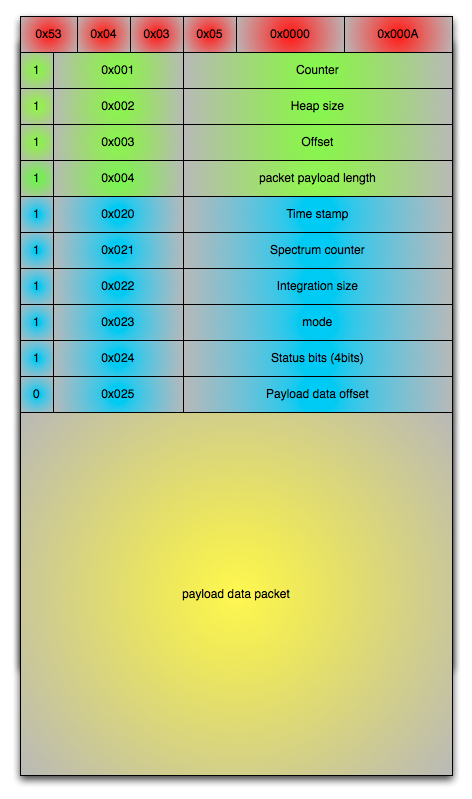
\includegraphics[width=7cm]{figures/spead_format_high_bandwidth.png}
\caption{Format of SPEAD packets for high-bandwidth modes}
\label{spead-hbw}
\end{figure}

\begin{figure}[!ht]
\centering
\includegraphics*[width=12cm, viewport = 50 291 540 705, page=1]{figures/spead_format_low_bandwidth.pdf}
\caption{Format of SPEAD packets for high-bandwidth modes (multiple subbands)}
\label{spead-lbw-multiple}
\end{figure}

\begin{figure}[!ht]
\centering
\includegraphics*[width=9cm, viewport = 100 295 500 705, page=2]{figures/spead_format_low_bandwidth.pdf}
\caption{Format of SPEAD packets for low-bandwidth modes (single subband)}
\label{spead-lbw-single}
\end{figure}

The header fields for the various packet formats are explained below:
\begin{itemize}
\item {\bf Heap counter:} in high-bandwidth modes, each heap represents a single spectrum. Therefore, a heap may be multiple packets long. In low-bandwidth modes, a heap is just a single packet containing a set of time samples.
\item {\bf Heap size:} the size of the heap (which may be multiple packets), in bytes.
\item {\bf Heap offset:} if the heap is multiple packets long (as in high-bandwidth modes), the offset field indicates where this packet's payload fits into the larger heap.
\item {\bf Packet payload length:} length of this packet's payload data, in bytes.
\item {\bf Time counter:} this counter is incremented at the FPGA  clock rate. The field records the FPGA time counter at the clock cycle when spectrum is outputted from the PFB (high-bandwidth modes) or when the time samples are recorded (low-bandwidth modes). It is reset at the 1 PPS tick after an ARM command is issued.
\item {\bf Spectrum counter:} this counter is incremented every spectrum, even blanked spectra. It counts the spectra coming out of the PFB. It is reset at the 1 PPS tick after an ARM command is issued.
\item {\bf Integration size:} this counter is incremented every spectrum, unless that spectrum is blanked. It is reset at the start of each FPGA integration. This counter therefore indicates the number of spectra that were integrated on the FPGA, before the integrated spectrum was transmitted to the HPC. For most packets, this counter has the value FPGA\_NMAX\_SPECTRA. However, if the status bits change during the integration, this counter value will be less than FPGA\_NMAX\_SPECTRA.
\item {\bf Mode:} the mode in which the FPGA is operating (a number from 1 to 17).
\item {\bf Status bits:} the state if the three switching signals and the blanking signal. Bit 3 is the blanking signal, while bits 2 to 0 are the calibration, position and frequency switching signals.
\item {\bf Payload data offset: } the number of bytes between the end of the {\em Packet payload length} field and the beginning of the payload data section, in this packet.
\end{itemize}

\subsubsection{The Payload Data Field for High-Bandwidth Modes}
As mentioned, a single spectrum (or heap) may be split over multiple SPEAD packets. Within the {\em Payload Data} field of a single packet, the data is stored as follows:
\begin{verbatim}
Ch0_XX*, Ch0_YY*, Re(Ch0_X*Y), Im(Ch0_X*Y),
Ch1_XX*, Ch1_YY*, Re(Ch1_X*Y), Im(Ch1_X*Y),
…
Ch2047_XX*, Ch2047_YY*, Re(Ch2047_X*Y), Im(Ch2047_X*Y)
\end{verbatim}

Note that each value is a 32-bit signed integer. \texttt{Ch[0-2047]} represents the spectral channel. For modes where only 1024 spectral channels are used, the packet will only be 4kB long.

\texttt{XX*} is a real number and represents the power in X plane. \texttt{YY*} is a real number and represents the power in Y plane. \texttt{X*Y} is a complex number and represents the cross-correlation. \texttt{XY*} is not transmitted.

\subsubsection{The Payload Data Field for Low-Bandwidth Modes (multiple subbands)}
A heap is always one packet long in these modes. Therefore, the heap counter is the same as the packet counter, and the heap offset is always zero.

The ordering of the data within the payload is indicated in the diagram above. For example, \texttt{Sub0\_PolA\_Re\_0} is interpreted as: \\
\texttt{Sub0} = sub-band 0 \\
\texttt{PolA} = polarisation A \\ 
\texttt{Re} = the real component of the signal \\
\texttt{0} = sample at time instant 0

Each packet therefore contains samples from 256 time instances and 8 different sub-bands.

Finally, the centre frequencies and bandwidth of each sub-band are not stored in the packet header. They are instead passed to the HPC software via the status shared memory.

\subsubsection{The Payload Data Field for High-Bandwidth Modes (single subband)}
A heap is always one packet long in these modes. Therefore, the heap counter is the same as the packet counter, and the heap offset is always zero.

The ordering of the data within the payload is indicated in the diagram above. For example, \texttt{PolA\_Re\_0} is interpreted as: \\
\texttt{PolA} = polarisation A \\
\texttt{Re} = the real component of the signal \\
\texttt{0} = sample at time instant 0

Each packet therefore contains samples from 2048 time instances.

\subsection{Structure of the Shared Memory Data Buffers}
\label{data-buffer-section}

As described earlier, the shared memory data buffers are used to pass time/frequency samples from one thread to another. Each data buffer is in fact a ring buffer, containing a number of independent blocks protected by semaphores. All three shared memory data buffers have the following common structure, as shown in Figure~\ref{vegas-buffer}:

\begin{figure}[!ht]
\centering
\includegraphics*[width=7cm, viewport = 80 270 360 780]{figures/vegas-buffer.pdf}
\caption{Structure of the Data Buffers}
\label{vegas-buffer}
\end{figure}

The {\bf guppi\_databuf structure} stores the size of the FITS header blocks, the indexes and the data blocks. It also keeps count of the number of data blocks within the buffer. Finally, it contains the semaphore ID for the shared memory buffer.

The {\bf FITS header} contains a snapshot of the status shared memory buffer, taken at the time that the network packets were first written to the corresponding data block. This means that the FITS header stores information such as antenna position, local machine timestamps and number of frequency channels. There is one FITS header for each data block, and each header is 184~320 bytes.

The {\bf index} is used for locating individual spectra within a single data block. There is one index per data block.

The {\bf data blocks} store the actual time samples or integrated spectra. The size of a single data block can vary, but it is typically 32MB in size. There are also typically 64 data blocks per buffer.

The contents of the data blocks and indexes do however vary, depending on the buffer type. These are described in the following sections.

\subsection{Structure of the Buffer at Input to the GPU or CPU Thread}

The shared memory data buffers at the input to the GPU and CPU accumulation threads store individual SPEAD heaps. Each heap contains a complete spectrum (CPU input buffer) or a block of consecutive time samples (GPU input buffer), along with associated meta data. Since there are typically a few hundred heaps per data block, and index is used to access individual heaps within a single data block. The structure of the index is shown in Figure~\ref{vegas-cpu-gpu-index}.

\begin{figure}[!ht]
\centering
\includegraphics*[width=12cm, viewport = 80 570 520 746]{figures/vegas-cpu-gpu-index.pdf}
\caption{Index for a {\em single} data block in the CPU and GPU input buffers}
\label{vegas-cpu-gpu-index}
\end{figure}

Although the index supports up to 4096 heaps per data block, the actual number of heaps within the block may be considerably less. All heaps within a block are of identical size. Each heap has an associated {\em heap counter}, {\em heap valid} flag and {\em MJD time} within the index. Consecutive heaps should have incrementing {\em heap counters}, except when the ARM signal occurs (then the {\em heap counter} is reset to zero). If a heap contains a corrupted packet, it is marked as invalid ({\em heap valid} = 0); otherwise the {\em heap valid flag} is set to 1. The {\em MJD time} field records the time (in 64-bit Modified Julian Date format with sub-second resolution) that the first network packet in that spectrum was received by the HPC.

Each data block simply contains many heaps, arranged one after the other, without any inter-heap space. The structure of a single heap is different for the GPU and CPU input buffers. These heap structures are described below.

\subsubsection{GPU Heap}

A single data block in the GPU buffer contains many GPU heaps. A single heap is simply a SPEAD packet for low-bandwidth VEGAS modes, with the SPEAD packet headers removed. A heap is therefore always one packet long in these modes. One such heap is shown in Figure~\ref{vegas-gpu-heap}.

\begin{figure}[!ht]
\centering
\includegraphics*[width=13cm, viewport = 55 410 540 760]{figures/vegas-gpu-heap.pdf}
\caption{A single heap within the GPU shared memory data buffer}
\label{vegas-gpu-heap}
\end{figure}

Each heap has four header fields that were described in Section~\ref{spead-section}. The ordering of the time samples within the heap is indicated in Figure~\ref{vegas-gpu-heap}. For example, \texttt{Sub0\_PolA\_Re\_0} is interpreted as:\\
\texttt{Sub0}	= sub-band 0\\
\texttt{PolA}	= polarisation A\\
\texttt{Re}	= the real component of the signal\\
\texttt{0}	= sample at time instant 0\\

Each heap therefore contains samples from 256 time instances and 8 different sub-bands; or from 2048 time instances in just 1 sub-band, depending on the mode.

\subsubsection{CPU Heap}

Each data block in the CPU input buffer contains multiple heaps. Each heap contains a complete 1ms-integrated spectrum in single sub-band modes, or 8 complete 1ms-integrated spectra in 8 sub-band modes. The structure of a single heap is shown in Figure~\ref{vegas-cpu-heap}.

\begin{figure}[!ht]
\centering
\includegraphics*[width=9cm, viewport = 120 420 470 765]{figures/vegas-cpu-heap.pdf}
\caption{A single heap within the CPU shared memory data buffer}
\label{vegas-cpu-heap}
\end{figure}

Each heap has a number of header fields, as described in Section~\ref{spead-section}. The structure of the spectrum data within the payload section of the heap is also described in Section~\ref{spead-section}. The size of a single heap depends on the number of sub-bands and spectral channels.

\subsection{Structure of the Buffer at Input to the Disk Thread}

The shared memory buffer at the input to the disk thread stores integrated spectra that are ready to be written to disk. Timestamps, frequency information and switching signal state information are also included for each integrated spectra. A single spectrum (or set of 8 spectra, in the modes where 8 sub-bands are used) is called a {\em data array}. The meta data associated with a single data array is stored in a \texttt{fits\_data\_columns} structure. Since a single data block may contain hundreds of data arrays and structures, an index is used to access each spectrum. The index for a single data block in disk shared memory buffer is shown in Figure~\ref{vegas-disk-index}.

\begin{figure}[!ht]
\centering
\includegraphics*[width=11cm, viewport = 80 650 460 790]{figures/vegas-disk-index.pdf}
\caption{Index for a {\em single} data block in the disk input buffer}
\label{vegas-disk-index}
\end{figure}

A dataset is defined as an instance of the \texttt{fits\_data\_columns} structure, followed by the associated spectral data (the data array). The index supports up to 8192 datasets, but again the actual number of datasets within a data block may be less. The size of a single data array is specified within the index, as it depends on the number of frequency channels. The size of the \texttt{fits\_data\_columns} structure is always fixed.

The offset fields, in the index, indicate the relative position of the start of the specified structure or data array. The offset is defined as the number of bytes from the beginning of the data block (and not from the beginning of the data buffer).

The actual data block itself simply contains many datasets, one after the other. As mentioned, a dataset is a structure followed by a data array. C code for the \texttt{fits\_data\_columns} structure is given below. Note that the \texttt{accumid} field has a value from 0 to 7, indicating the state of the switching signals for this integration.

\begin{verbatim}
struct sdfits_data_columns
{
    double time;            // MJD at start of integration (from Linux time)
    int time_counter;       // FPGA time counter at start of integration
    int integ_num;          // The integration number (a specific integ. period)
    float exposure;         // Effective integration time (seconds)
    char object[16];        // Object being viewed
    float azimuth;          // Commanded azimuth
    float elevation;        // Commanded elevation
    float bmaj;             // Beam major axis length (deg)
    float bmin;             // Beam minor axis length (deg)
    float bpa;              // Beam position angle (deg)

    int accumid;            // ID of the accumulator from where spectrum came
    int sttspec;            // SPECTRUM_COUNT of first spectrum in integration
    int stpspec;            // SPECTRUM_COUNT of last spectrum in integration

    float centre_freq_idx;  // Index of the NCHAN/2 frequency bin (0-indexed)
    double centre_freq[8];  // Frequency at centre of each sub-band
    double ra;              // RA mid-integration
    double dec;             // DEC mid-integration

    char data_len[16];      // Length of the data array
    char data_dims[16];     // Data matrix dimensions
    unsigned char *data;    // Ptr to the raw data (used internally only)
};
\end{verbatim}

The {\em data array} can be regarded as a 3-dimensional array of floats, with the following structure:

\texttt{float data[NUM\_SUBBANDS][NUM\_CHANS][NUM\_STOKES]}
\\
where: \\
NUM\_SUBBANDS = number of sub-bands specified mode [1 - 8] \\
NUM\_SUBCHANS = number of frequency channels/bins [1024 - 32768] \\
NUM\_STOKES = 4.

The number of sub-bands and number of frequency channels can be obtained from the FITS header for the data block (see section \ref{data-buffer-section}).

\subsection{Status Shared Memory Buffer}

The status shared memory buffer stores a number of variables in FITS format (i.e. as ASCII strings in 80-character fields). The buffer should therefore be read and written using a FITS-compatible reader. The fields in Table~\ref{status-buffer-critical} must be set before the VEGAS HPC software is started, as these fields affect how the software operates. Note that these are all input parameters.

It is recommended that a script be used to set these parameters, according to the observation mode. See {\em Memo on the Critical Settings for the HPC} for the recommended values for these parameters, for each operating mode.

\begin{table}[!h]
\centering
\caption{Status Buffer Fields for Critical Settings [Inputs]}
\begin{tabular}{l l l}
\hline
\bf Field Name & \bf Data Type & \bf Description \\
\hline
NSUBBAND & Integer & Number of sub-bands (1 to 8) \\
NPOL & Integer & Number of antenna polarisations (must be 2) \\
NCHAN & Integer &  Number of frequency channels per sub-band \\
CHAN\_BW & Double & Width of each spectral channel/bin [Hz]\\
EXPOSURE & Float & Required integration time [s] \\
HWEXPOSR & Float & Hardware integration time (on FPGA or GPU) [s]\\
FPGACLK & Float & FPGA clock rate [Hz] \\
EFSAMPFR & Float & Effective sampling frequency (after decimation) [Hz] \\
SUB0FREQ & Double & Centre frequency of sub-band 0 [Hz] \\
SUB1FREQ & Double & Centre frequency of sub-band 1 [Hz] \\
SUB2FREQ & Double & Centre frequency of sub-band 2 [Hz] \\
SUB3FREQ & Double & Centre frequency of sub-band 3 [Hz] \\
SUB4FREQ & Double & Centre frequency of sub-band 4 [Hz] \\
SUB5FREQ & Double & Centre frequency of sub-band 5 [Hz] \\
SUB6FREQ & Double & Centre frequency of sub-band 6 [Hz] \\
SUB7FREQ & Double & Centre frequency of sub-band 7 [Hz] \\
DATAHOST & String & Hostname of attached ROACH board \\
DATAPORT & Integer & UDP port to which ROACH board transmits packets \\
PKTFMT & String &  Network packet format (must be SPEAD) \\
DATADIR & String & FITS output directory (only when disk thread used) \\
FILENUM & Integer & File number in multi-file scan (reset to zero for each scan) \\
\hline
\end{tabular}
\label{status-buffer-critical}
\end{table}

The fields in Table~\ref{status-buffer-telescope} are the telescope observation parameters, that are read from the M\&C server. These fields are written to the Disk shared memory buffer, so that they can be written to the output FITS file. Therefore, none of these parameters are actually used by the HPC software. Again, these parameters are all inputs to the software.

\begin{table}[!h]
\centering
\caption{Status Buffer Fields for Telescope Parameters [Inputs]}
\begin{tabular}{l l l l}
\hline
\bf Field Name & \bf Data Type & \bf Description \\
\hline
TELESCOP & String & Name of telescope \\
PROJID & String & Project ID  No \\
OBSFREQ & Double & Centre frequency of observation [Hz] \\
OBSBW & Double & Entire backend bandwidth for observation [Hz] \\
OBSNCHAN & Double & Number of original frequency channels/bins \\
FRONTEND & String & Name of observation frontend \\
INSTRUME & String & Name of observation backend (always "VEGAS") \\
SCANNUM & Integer & Scan number in single observation \\
OBJECT & String & Object being viewed \\
STTMJD & Double & Commanded observation start time [MJD double] \\
TSYS & Double & System temperature \\
FILTNEP & Float & Filter noise-equivalent parameter (noise of PFB) \\
AZ & Float & Commanded azimuth [deg] \\
ELEV & Float & Commanded elevation [deg] \\
RA & Double & Right-ascension [deg] \\
DEC & Double & Declination [deg] \\
BMAJ & Float & Beam major-axis length [deg] \\
BMIN & Float & Beam minor-axis length [deg] \\
BPA & Float & Beam position angle [deg] \\
CAL\_MODE & String & Calibration mode (OFF, SYNC, EXT) \\
CAL\_FREQ & Double & Calibration modulation  frequency [Hz] \\
CAL\_DCYC & Double & Calibration duty cycle \\
CAL\_PHS & Double & Calibration phase (w.r.t. start time) \\
\hline
\end{tabular}
\label{status-buffer-telescope}
\end{table}

Table \ref{status-buffer-monitor} gives the output fields that indicate the status of the HPC software. These fields are written by the HPC software, and can be monitored by an external application. Most of these fields are self explanatory, with the possible exception of the status fields (NETSTAT, etc). These fields will typically take one of the following values: ``init'', ``waiting'' (for incoming data), ``receiving'' (network packets), ``processing'', ``blocked'' (no output block available) and ``writing'' (to disk).

The *BLKIN and *BLKOU fields indicate to/from which block (in a particular ring buffer) each thread is writing/reading. For a 24 block ring buffer, the blocks would have the ID numbers 0 to 23. These fields allow the number of free blocks in each ring buffer to be calculated in realtime, and hence identify any potential problems. For example, to calculate the number of {\em filled} blocks in the disk buffer, use:

\texttt{(PFBBLKOU - DSKBLKIN) \% NUM\_BLOCKS\_IN\_BUF}.

\begin{table}[!h]
\centering
\caption{Status Buffer Fields for Reporting on Status of HPC Software [Outputs]}
\begin{tabular}{l l l}
\hline
\bf Field Name & \bf Data Type & \bf Description \\
\hline
NPKT & Integer & Number of packets received from ROACH \\ 
NDROP & Integer & Number of packets dropped \\ 
DROPAVG & Double & Current packet drop rate \\ 
DROPTOT & Double & Overall packet drop rate \\
NETSTAT & String & Status of network thread \\
GPUSTAT & String & Status of GPU thread \\
ACCSTAT & String & Status of CPU accumulator thread \\
DISKSTAT & String & Status of disk thread \\
NETBLKOU & Integer & ID number of current output block for network thread \\ 
PFBBLKIN & Integer & ID number of current input block for PFB thread \\ 
PFBBLKOU & Integer & ID number of current output block for PFB thread\\ 
ACCBLKIN & Integer & ID number of current input block for accumulator thread\\ 
ACCBLKOU & Integer & ID number of current output block for accumulator thread\\ 
DSKBLKIN & Integer & ID number of current input block for disk thread \\
DSKEXPWR & Integer & The number of exposures written to disk \\ 
M\_STTMJD & Double & Measured observation start time (MJD; microsec resolution)\\
M\_STTOFF & Double & Measured observation start time offset (fraction of second) \\
SWVER & String & Version number of the VEGAS HPC software \\
\hline
\end{tabular}
\label{status-buffer-monitor}
\end{table}

\subsubsection{Programmatic Access to the Shared Memory Segments}

The shared memory segments can be programmatically accessed using their keys.
The following description applies to the dual-instance version of VEGAS.

On a PC on which dual-instance shared memory is set up, running {\tt ipcs}
should show something similar to the following:

\begin{verbatim}
------ Shared Memory Segments --------
key        shmid      owner      perms      bytes      nattch     status      
0x4019ccf5 131072     owner      666        184320     0                       
0x8019ccf5 163841     owner      666        1081745664 0                       
0x8019ccf6 196610     owner      666        1081745664 0                       
0x8019ccf7 229379     owner      666        408658112  0                       
0x4119ccf5 262148     owner      666        184320     0                       
0x8119ccf5 294917     owner      666        1081745664 0                       
0x8119ccf6 327686     owner      666        1081745664 0                       
0x8119ccf7 360455     owner      666        408658112  0                       

------ Semaphore Arrays --------
key        semid      owner      perms      nsems     
0x8019ccf5 65538      owner      666        32        
0x8019ccf6 98307      owner      666        32        
0x8019ccf7 131076     owner      666        1024      
0x8119ccf5 163845     owner      666        32        
0x8119ccf6 196614     owner      666        32        
0x8119ccf7 229383     owner      666        1024      
\end{verbatim}

The first four shared memory segments and the first three semaphores correspond
to instance 0, with the rest corresponding to instance 1. The key generation
functionality is implemented in the files {\tt vegas\_ipckey.c} and {\tt vegas\_ipckey.h}.
Keys are generated using the {\tt ftok()} function (see manpage), which takes a {\tt proj\_id}
built in the following way:

For data buffers, {\tt proj\_id = (instance\_id \& 0x3f) | 0x80}, and for status buffers,
{\tt proj\_id = (instance\_id \& 0x3f) | 0x40}. For instance IDs 0 and 1, this would correspond to
{\tt 0x80} and {\tt 0x81} respectively for data buffers and {\tt 0x40} and {\tt 0x41} respectively
for status buffers. That is, the keys starting with {\tt 0x40} and {\tt 0x80} correspond to instance 0,
and those starting with {\tt 0x41} and {\tt 0x81} correspond to instance 1.

The instance ID is passed as a command-line argument to {\tt vegas\_hpc\_hbw} and {\tt vegas\_hpc\_lbw},
and this is used by their processes to attach themselves to the relevant shared memory segments and use
the relevant semaphores, as demonstrated by the following example:

\begin{verbatim}
struct vegas_status st;
rv = vegas_status_attach(instance_id, &st);
...
struct vegas_databuf *db;
db = vegas_databuf_attach(instance_id, args->output_buffer);
\end{verbatim}


%%%%%%%%%%%%%%%%%%%%%%%%%%%%%%%%%%%%%%%%%%%%%
% CHAPTER: PROCESSING THREADS
%%%%%%%%%%%%%%%%%%%%%%%%%%%%%%%%%%%%%%%%%%%%%

\clearpage
\section{The CPU-based HPC Processing Threads}

In this section, the four data processing threads within the VEGAS HPC software, that run on the CPU, will be discussed. Since the GPU Thread operates quite differently to the other four threads, it is described separately in Section~\ref{gpu-section}.

\subsection{The Main Threads}
The two ``main'' threads are \texttt{vegas\_hpc\_hbw} and \texttt{vegas\_hpc\_lbw}. These threads are responsible for starting the data processing threads depicted in Figures~\ref{vegas-buffers-nogpu} and \ref{vegas-buffers-gpu}. Note that only one of these two threads never run simultaneously.

These two threads first attempt to attach to the shared data buffers. If they do not exist yet, they are created with default block sizes. The data blocks in the disk input buffer are then resized according to the EXPOSURE parameter (see below for more details). The network, PFB, accumulator and disk threads are then launched. Depending on the mode and command line parameters, not all four threads may be launched.

The main thread then waits for the global variable \texttt{run} to be set to zero. This happens if an error occurs in one of the data processing threads, or if the user presses Control-C. In either case, the main thread kills all the other threads and closes the program.

\subsubsection{Dynamic Block Resizing}
If the data blocks in the disk input buffer are large, and a long integration time is used, data blocks will be written to hard disk very infrequently (possibly only once an hour). This means that if the program were to crash, up to an hour of data could be lost. To prevent this, the main thread resizes the data blocks in the disk input buffer so that these data blocks fill up every 20 seconds.

The size of the blocks in the disk buffer are calculated as follows (where EXPOSURE, NCHAN and NSUBBAND are all parameters that are set via the status shared memory):

\begin{verbatim}
  DISK_WRITE_INTERVAL = 20 seconds
  num_exp_per_blk = DISK_WRITE_INTERVAL / EXPOSURE
  exposure_data_size = NCHAN * NSUBBAND * 4 * 4
  disk_block_size = num_exp_per_blk * exposure_data_size
  disk_block_size = min(disk_block_size, 32*1024*1024)
\end{verbatim}

The last step ensures that the disk block size does not exceed 32MB. Once the calculation is done, the disk buffer is then reconfigured so that it uses the new block size. The number of data blocks in the buffer is adjusted accordingly, so that the overall buffer size remains constant (as determined by the initial user configuration).

When the buffers are first created (typically using the scripts), an array of 1024 semaphores is created for the disk input buffer. This therefore limits the number of blocks per buffer to 1024. Typically, there will be far less than 1024 blocks in the disk buffer, resulting in only a few of the 1024 semaphores being used. However, if the resizing operation results in blocks that are very small, causing there to be more than 1024 buffer blocks, this will be limited to 1024 blocks, resulting in a reduction in the overall disk buffer size.

\subsection{Operations Common to all Four Data Processing Threads}

The four data processing threads, described in the sections below, have common initialization operations. These common operations are:

\begin{enumerate}
\item Each thread sets its CPU affinity, so that each thread runs on a different physical processor. Since the target processor uses hyperthreading, this means that each thread is allocated to every second CPU.
\item The thread then attaches to the status shared memory, and reads the parameters from the shared memory into \texttt{vegas\_params} and \texttt{sdfits} structures. This allows the thread to configure its internal operations according to the parameters in the status shared memory.
\item The thread attaches to its input and output shared data buffers.
\item The thread then enters an infinite loop in which the actual work is done. This loop terminates when one of the threads sets the global \texttt{run} variable to zero.
\end{enumerate}

\subsection{The Network Thread}

The network thread performs the following main operations in its processing loop:
\begin{enumerate}
\item Waits for a UDP packet to arrive, using the Linux \texttt{poll} command.
\item The packet is checked to ensure that it has a valid header, and that the packet is the correct length.
\item The \emph{heap counter} and \emph{heap offset} fields are combined to form a unique packet number. This packet number is compared to the packet number of the previously received packet. If the packet number decreased by more than 1024, then the observation begins (i.e. the ARM signal was sent to the FPGA, causing the FPGA to reset its heap counter).
\item If the packet number is the same as the previously received packet, the packet is discarded (duplicate packet). If the packet number is slightly smaller than the previous packet, the packets were sent out of order, and are discarded.
\item If the software has not yet detected the start of the observation (as indicated by the condition in point 3), the packet is discarded. If the observation has begun, the packet is processed according to the following steps.
\item The received packet is then written into the CPU or GPU input buffer (depending on the mode). Within a particular data block in the buffer, all the SPEAD headers (excluding the first 40 bytes) are placed at the beginning, while the payloads are placed at the end. This is to allow fast bulk-copying of data onto the GPU.

Note that the GPU and CPU buffers store heaps, and not buffers. This means that in high-bandwidth modes, all the packets that form a single heap (i.e. single spectrum) will have just one SPEAD header, and all their payloads will be concatenated together to form a single block of spectral data. Furthermore, in high-bandwidth modes, the byte ordering of the floating-point numbers is reversed when writing the data to the CPU input buffers, to correct the endianess.. 
\item The index is also updated with the {\em heap counter}, the MJD time (obtained from Linux time) and whether any packets were dropped within this heap ({\em valid} flag).
\item If the buffer block is not yet full, go to Step 1. If however the buffer block is full, the semaphore corresponding to that block in the shared semaphore array is set, informing the next thread that it can process the data in the block. The network thread then waits for an empty block to become available in the GPU or CPU input buffer, before going to Step 1.
\end{enumerate}

\subsection{The PFB Thread}

The main loop in the \texttt{vegas\_pfb\_thread.c} file simply waits for data blocks in the GPU input buffer to become available. Whenever one becomes available, it calls the \texttt{do\_pfb(...)} function in the GPU code with a pointer to the data block. When the function returns, it marks the input block as available (so that the network thread can refill it at some later point) and then goes back to waiting for another input block.

\subsection{The CPU Accumulator Thread}

Before entering the main processing loop, \texttt{vegas\_accum\_thread.c} dynamically allocates memory for the 8 vector accumulators (one for each switching state). The 8 vector accumulators are stored as a 2D floating-point array that can be described by:
\begin{verbatim}
float accumulator[NUM_SW_STATES][num_chan * num_subband * NUM_STOKES]
\end{verbatim}

Note that the accumulators always store floating-point numbers, and that \texttt{NUM\_SW\_STATES~=~8}. Even though the vector accumulators are stored as a single 2D array, they are logically indexed as a 4D array with the following structure:

\begin{verbatim}
float accumulator[NUM_SW_STATES][num_chan][num_subband][NUM_STOKES]
\end{verbatim}

There are also two other arrays that are associated with the accumulators:
\begin{verbatim}
char accum_dirty[NUM_SW_STATES]
struct sdfits_data_columns data_cols[NUM_SW_STATES]
\end{verbatim}

The \texttt{accum\_dirty} array stores flags indicating whether a particular accumulator has had anything added to it this integration cycle. The \texttt{data\_cols} array stores the metadata associated with each integrated spectrum, such as the timestamp at the start of the integration, the total integration time and the antenna position.

After these additional initialization steps, the CPU Accumulator Thread enters its main loop, performing the following steps:

\begin{enumerate}

\item Wait for a block in the CPU Input shared memory buffer to become full.
\item For each heap in the input buffer block:

\begin{enumerate}
\item If the heap is marked as bad (invalid) in the index in the CPU input buffer, it is ignored. Also, if the blanking bit is high (bit 3 of \emph{Status bits} field in SPEAD heap header), the heap is ignored.
\item Provided the heap is not ignored, it is added to one of the 8 vector accumulators, based on bits 2:0 of the \emph{Status bits} field in SPEAD heap header. In the case of high-bandwidth modes (where the FFT is done on FPGA), the 32-bit integers are converted to 32-bit floats before being adding to the accumulators.
\item If the accumulator was all zeroes before adding this heap (spectrum), the dirty bit for that accumulator is set. The timestamp for the integration is also set using the timestamp from the input heap. This means that the vector accumulator (for that particular switching state) has the timestamp of the first spectrum in the accumulation.
\item The total accumulation time (\texttt{accum\_time}) for this integration cycle is updated using:
\begin{verbatim}
pfb_rate = EFSAMPFR / (2 * NCHAN)
accum_time += integ_size / pfb_rate
\end{verbatim}
where EFSAMPFR is the effective sampling frequency of the FPGA (set via status shared memory), NCHAN is the number of channels in the FFT (also set via the status shared memory), and \texttt{integ\_size} is the number of spectra that were added together, in either the FPGA or the GPU, to produce the input heap (spectrum). The \texttt{integ\_size} parameter is obtained from the SPEAD header of the input heap.
\item The exposure for that particular vector accumulator is also increased, using the same formula as above.
\item If the total \texttt{accum\_time} $\ge$ EXPOSURE (i.e. the EXPOSURE parameter in the status shared memory), all the {\em dirty} accumulators are written to the output buffer (i.e. the Disk input buffer). Each dirty accumulator is written as a separate dataset, with its own \texttt{fits\_data\_columns} structure and data array, to the disk input buffer. Non-dirty accumulators are not written. All the dirty accumulators are then zeroed out for the start of the next integration cycle.
\end{enumerate}

\item The block in the CPU input buffer is marked as free, so that it can be reused by the Network Thread or PFB Thread at some later time.
\item Go to Step 1.

\end{enumerate}

\subsection{The Disk Thread}

The disk thread performs the following main operations in its processing loop:
\begin{enumerate}
\item Wait for a block in the Disk Input shared memory buffer to become full.
\item Each dataset in the input buffer block is passed to the \texttt{sdfits\_write\_subint} function, which writes that particular dataset to the SDFITS output file. Note that each dataset appears as a separate, single line in the SDFITS output file.
\item The block in the Disk input buffer is marked as free, so that it can be reused by the CPU Accumulation Thread at some later time.
\item Go to Step 1.
\end{enumerate}


%%%%%%%%%%%%%%%%%%%%%%%%%%%%%%%%%%%%%%%%%%%%%
% CHAPTER: GPU
%%%%%%%%%%%%%%%%%%%%%%%%%%%%%%%%%%%%%%%%%%%%%

\clearpage
\section{The GPU Thread}
\label{gpu-section}

The GPU thread is instantiated only for the low-bandwidth modes of operation of
VEGAS. The GPU thread reads data from the GPU buffer, performs PFB/FFT and
accumulation for 1ms, and writes the accumulated spectra to the CPU buffer for
the consumption of the CPU thread.

\subsection{Files}

The following are the files relevant to the GPU thread. In {\tt \$VEGAS/vegas\_hpc/src}:

\vspace{11pt}

\noindent
{\tt vegas\_pfb\_thread.c}: Entry point of the GPU thread\\
{\tt pfb\_gpu.cu}: Host functions\\
{\tt pfb\_gpu.h}: Host functions header file\\
{\tt pfb\_gpu\_kernels.cu}: Device kernels\\
{\tt pfb\_gpu\_kernels.h}: Device kernels header file\\

In {\tt \$VEGAS/gpu\_dev}:

\vspace{11pt}

\noindent
{\tt vegas\_gencoeff.py}: Filter coefficient generation script

\subsection{Code Flow}

The basic code flow of the GPU thread is listed below. Here, `host' refers to
CPU/RAM and `device' refers to GPU/associated memory. The term `kernel' refers
to the CUDA/C function that runs on the GPU. For further details on CUDA
programming, see the \href{http://www.nvidia.com/object/cuda_home_new.html}{NVIDIA CUDA C Programming Guide}. 

\begin{enumerate}
  \item Initialization ({\tt pfb\_gpu.cu}: {\tt init\_gpu()})
    \begin{enumerate}
      \item Choose a CUDA device (hardcoded to device 0).
      \item Get device properties.
      \item Allocate memory for filter coefficients array, read filter
            coefficients file (see \S\ref{filtercoeff}), and load values.
      \item Allocate memory for data arrays.
      \item Calculate CUDA kernel parameters.
      \item Create FFT plan (one plan for all FFTs, using {\tt cufftPlanMany()}).
    \end{enumerate}
  \item Set status to `waiting' and wait for input data buffer to fill up.
  \item Set status to `processing' and process data ({\tt pfb\_gpu.cu}: {\tt do\_pfb()}).
    \begin{enumerate}
      \item Copy entire data in current input block to device.
      \item If all heaps that go into one PFB operation ({\tt VEGAS\_NUM\_TAPS * g\_iNumSubBands * g\_nchan} samples)
            are valid, perform polyphase filtering (for details of the algorithm, see the
            \href{https://casper.berkeley.edu/wiki/The_Polyphase_Filter_Bank_Technique}
            {CASPER Memo on the PFB technique}). If there is any invalid heap,
            skip all heaps that go into this PFB.
      \item Perform FFTs. All FFTs (2 for the 1-sub-band modes, and 16 for the 8-sub-band modes)
            are executed in parallel.
      \item If the blanking bit is not set, accumulate for 1ms, copy the accumulated
            spectrum back to the host, and write it to the CPU buffer. If the
            blanking bit just turned on, copy whatever has been accumulated till then
            back to the host and dump it to the CPU buffer. Zero the accumulators.
      \item If the current output block is full, set status to `blocked' and wait
            for the next one to be available.
    \end{enumerate}
\end{enumerate}

The number of spectra to accumulate, corresponding to a time of 1ms, is
computed in {\tt vegas\_pfb\_thread.c} as
\begin{verbatim}
acc_len = abs(CHAN_BW) * HWEXPOSR
\end{verbatim}
where CHAN\_BW is the channel bandwidth and HWEXPOSR is the hardware
integration time, both of which are set by the user in the status shared memory.

The dual-polarization complex samples, that are interleaved as explained in the
previous sections, are read into a CUDA {\tt char4} array. To elaborate, if the
variable is named {\tt c4Data}, the four elements that make up this variable
would contain the following data:

\vspace{11pt}

\noindent
{\tt c4Data.x}: Real(X-pol.)\\
{\tt c4Data.y}: Imag(X-pol.)\\
{\tt c4Data.z}: Real(Y-pol.)\\
{\tt c4Data.w}: Imag(Y-pol.)

\vspace{11pt}

The spectra are written in the following format. The length of each block is
given in parentheses, in units of samples.
\begin{verbatim}
---------------------------------------------------
| PowX (1) | PowY (1) | Re(XY*) (1) | Im(XY*) (1) | (Interleaved samples)
---------------------------------------------------
\end{verbatim}


\subsection{Notes on Notation}

A quasi-Hungarian notation is used in most of the CUDA code. Example:

\begin{verbatim}
#define DEF_NFFT    1024    /* `DEF_' denotes default values */

int g_iVar; /* global variable */

<ret-type> Function(<args>)
{
    float fVar;
    int iVar;
    double dVar;

    /* CUDA types */
    char4 c4Var;
    float2 f2Var;
    dim3 dimVar;

    /* pointers */
    char *pcVar;
    int *piVar;

    /* arrays */
    float afVarArray[10];

    ...
}
\end{verbatim}


\subsection{PFB Filter Coefficients} \label{filtercoeff}

The PFB filter coefficients are read from a file during initialization. This
file is expected to be in the {\tt \$VEGAS/vegas\_hpc} directory.
Depending on the mode, the GPU thread needs to read in different sets
of coefficients, saved in different files. The file naming convention is as
follows. The file name is composed of different segments, each separated from
the neighbouring segments by an underscore, as shown below:\\
{\tt coeff\_<data-type>\_<taps>\_<nfft>\_<sub-bands>.dat}

The first segment is always the string `{\tt coeff}'. The second segment is the
data type of the coefficients, which, for the purpose of VEGAS, is always
single-precision floating point, and hence, `{\tt float}'. The third segment
is the number of taps of the PFB, followed by
the number of channels, and the number of sub-bands. As examples, the sets of
coefficients that VEGAS needs are pre-computed and saved in the following two
files:\\
{\tt coeff\_float\_8\_4096\_8.dat}: 8 taps, 4096 channels, 8 sub-bands (modes
13-17)\\
{\tt coeff\_float\_8\_32768\_1.dat}: 8 taps, 32768 channels, 1 sub-band (modes
6-12)

Generation of filter coefficients afresh is not necessary unless implementing
a new mode with a different number of channels and/or sub-bands, in which case,
the Python script {\tt vegas\_gencoeff.py} can be used for the purpose. The
usage of the script is as follows:

\begin{verbatim}
Usage: vegas_gencoeff.py [options]
    -h  --help                 Display this usage information
    -n  --nfft <value>         Number of points in FFT
    -t  --taps <value>         Number of taps in PFB
    -b  --sub-bands <value>    Number of sub-bands in data
    -d  --data-type <value>    Data type - "float" or "signedchar"
    -p  --no-plot              Do not plot coefficients
\end{verbatim}

The data type tells the program whether to output single-precision floating
point coefficients or signed chars in the range [-128, 127]. Note that
VEGAS can only accept single-precision floating point. The number of sub-bands
does not actually affect the coefficients themselves, but is included as an
optimization feature -- each coefficient repeats that many times, for ease of
GPU thread indexing. The output is a binary file.

This Python script requires the NumPy and matplotlib modules.

As for the values of the filter coefficients, they are generated in the
following manner:

\begin{verbatim}
M = NTaps * NFFT
X = numpy.array([(float(i) / NFFT) - (float(NTaps) / 2) for i in range(M)])
PFBCoeff = numpy.sinc(X) * numpy.hanning(M)
\end{verbatim}

That is, the coefficients array is a sinc function multiplied by a Hanning
window. This code can be modified, if needed, to create different sets of
coefficients.


\end{document}

